% Standalone figure: Fertility, BPE vs MorphBPE, all three languages.
% One metric per figure (split out of the former 3-panel groupplot, which
% read as too wide/cramped at single-column scale) -- each chart now gets
% full single-column real estate instead of a squeezed 5.2cm slot.
%
% Color: cyan = BPE, purple-blue = MorphBPE -- matches the source paper's
% own figure palette (colors sampled directly from its Figure 1), adjusted
% from the exact sampled hex values (#4FD2FF / #7B96EA) to pass CVD/contrast
% validation: those two were both too light against a white page and too
% close in hue to reliably separate under color-vision deficiency, however
% much the lightness was tuned. #0D9BD0/#8B5FDB keep the same cyan+purple-
% blue family and pass every check cleanly (see the dataviz skill's
% validator). Bars follow the dataviz mark spec: capped width, 4px rounded
% top / square baseline, no stroke (the 2px surface gap between bars does
% the separating, not a border), legend always present for 2 series,
% values labeled at the tip.
\documentclass[tikz]{standalone}
\usepackage{times}
\usepackage{pgfplots}
\pgfplotsset{compat=1.18}

\definecolor{seriesBPE}{HTML}{0D9BD0}
\definecolor{seriesMorphBPE}{HTML}{8B5FDB}
\definecolor{gridcolor}{HTML}{E1E0D9}
\definecolor{axiscolor}{HTML}{C3C2B7}
\definecolor{mutedtext}{HTML}{898781}
\definecolor{primaryink}{HTML}{0B0B0B}

\begin{document}
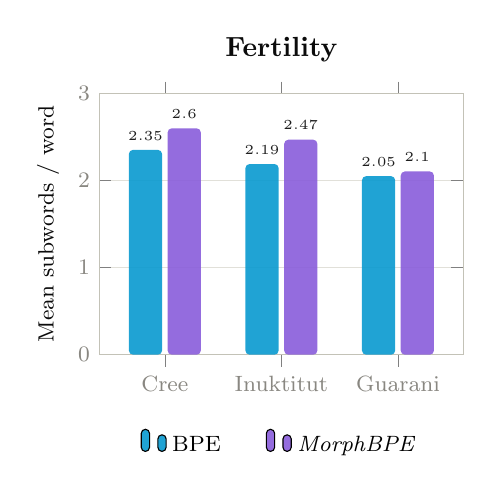
\begin{tikzpicture}
\begin{axis}[
    width=6.2cm, height=4.9cm,
    title={Fertility},
    title style={color=primaryink, font=\bfseries\normalsize, yshift=2pt},
    ybar,
    bar width=12pt,
    enlarge x limits=0.28,
    symbolic x coords={Cree,Inuktitut,Guarani},
    xtick=data,
    ymin=0, ymax=3.0,
    ylabel={Mean subwords / word},
    tick label style={color=mutedtext, font=\footnotesize},
    label style={color=primaryink, font=\footnotesize},
    axis line style={axiscolor},
    ymajorgrids=true,
    xmajorgrids=false,
    grid style={gridcolor, line width=0.5pt},
    every axis plot/.append style={draw=none, fill opacity=0.92, rounded corners=1.5pt},
    nodes near coords style={font=\tiny, color=primaryink},
    nodes near coords, every node near coord/.append style={/pgf/number format/.cd, fixed, precision=2},
    legend style={
        at={(0.5,-0.26)}, anchor=north,
        legend columns=-1,
        font=\footnotesize, draw=none, fill=none,
        /tikz/every even column/.append style={column sep=0.5cm},
    },
    legend cell align=left,
]
\addplot[fill=seriesBPE] coordinates {(Cree,2.351932428973637) (Inuktitut,2.189355277064774) (Guarani,2.050191264870318)};
\addlegendentry{BPE}
\addplot[fill=seriesMorphBPE] coordinates {(Cree,2.599180957256207) (Inuktitut,2.468730182696663) (Guarani,2.104207827147001)};
\addlegendentry{\textit{MorphBPE}}
\end{axis}
\end{tikzpicture}
\end{document}
